\documentclass[11pt]{article}
\usepackage{geometry, titlesec}
\usepackage[parfill]{parskip}
\usepackage[italicdiff]{physics}
\usepackage{amsfonts, amsthm}
\usepackage[cm]{fullpage}
\usepackage{fancyhdr}
\usepackage{xcolor}
\usepackage{siunitx, graphicx}
%\allowdisplaybreaks
 
%\renewcommand{\footrulewidth}{.2pt}
%\setlist[enumerate]{leftmargin=*}
\pagestyle{fancy}
\fancyhf{}
\lhead{Homework 2}
\rhead{Physics 133-B}
\setlength{\headheight}{11pt}
\setlength{\headsep}{11pt}
%\setlength{\footskip}{24pt}
%\cfoot{\today}
%\rfoot{\thepage}

\titleformat{\section}[runin]{\normalfont\large\bfseries}{Problem \thesection.}{1em}{}
\titleformat{\subsection}[runin]{\normalfont\large\bfseries}{\thesubsection}{1em}{}
\titleformat{\subparagraph}[leftmargin]{\normalfont\large\bfseries}{}{0pt}{}
\newcommand{\refeq}[1]{(\ref{#1})}

\newcommand{\beq}{\begin{equation*}}
\newcommand{\eeq}{\end{equation*}}

\newcommand{\beqn}{\begin{equation}}
\newcommand{\eeqn}{\end{equation}}

\newcommand{\qimplies}{\quad \implies \quad}


\newenvironment{statement}[1]
{
	\section{#1}
	\ignorespaces
}

\newenvironment{problem}
{
    \paragraph{Problem.}
    \color{darkgray}
    \ignorespaces
}

\newenvironment{solution}
{
    \paragraph{Solution.}
    \ignorespaces
}

\begin{document}

\newcommand{\dist}{\SI{2}{\meter}}
\newcommand{\freq}{\SI{800}{\Hz}}
\newcommand{\vsound}{\SI{344}{\meter\per\second}}
	

\begin{statement}{}
	Consider two speakers emitting sound at the same volume with frequency $f = \freq$.  One speaker is located at the origin, and the other on the $y$ axis at $y = \dist$.  At what locations on the positive $x$ axis is the interference completely constructive?  At what points is it completely destructive?
	
	Now we decrease $f$ until there are no longer any points of completely destructive interference on the positive $x$ axis.  How low must $f$ be for this to occur?
\end{statement}



\newcommand{\lam}{\lambda}
\newcommand{\ddA}{d_A}
\newcommand{\ddB}{d_B}
\newcommand{\Dely}{\Delta y}
\newcommand{\wavel}{\SI{0.43}{\meter}}

\begin{solution}
	Consider the setup shown below:
	
	\begin{center}
		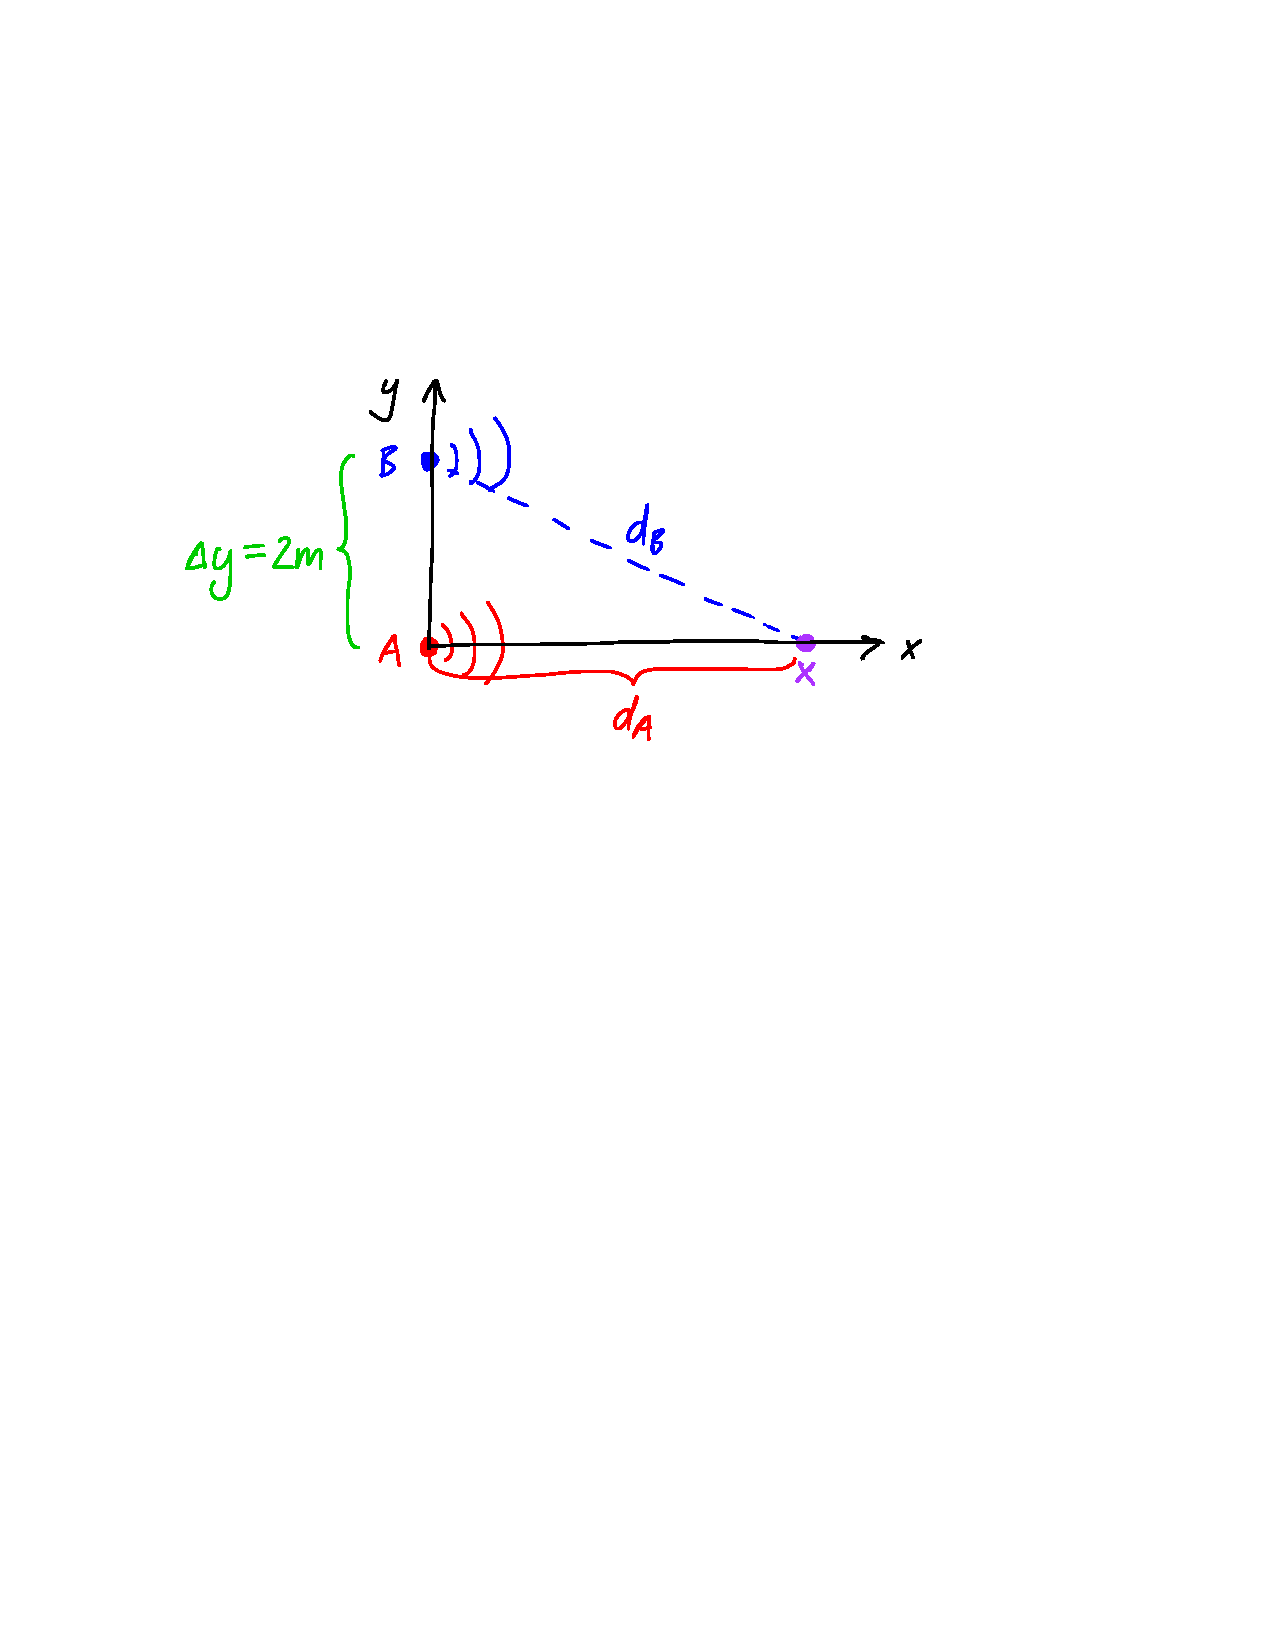
\includegraphics{fig1}
	\end{center}
	
	The path difference $d$ (which is called $\Delta x$ in the lecture slides) is given by
	\beq
		d = \ddB - \ddA = \ddA - x,
	\eeq
	and from trigonometry,
	\beq
		\ddB^2 = x^2 + (\Dely)^2
		\qimplies
		\ddB = \sqrt{x^2 + (\Dely)^2},
	\eeq
	where $\Dely$ is the distance between the two speakers.  Putting these together, we can write
	\beq
		d = \sqrt{x^2 + (\Dely)^2} - x.
	\eeq
	Completely constructive interference occurs where the interference pattern of the speakers has a maximum, which is when
	\begin{align*}
		d &= n \lam, &
		n &= 0, \pm 1, \pm 2, \ldots.
	\end{align*}
	Completely destructive interference occurs where it has a minimum, and
	\begin{align*}
		d &= \left( n + \frac{1}{2} \right) \lam, &
		n &= 0, \pm 1, \pm 2, \ldots.
	\end{align*}
	Recall that the wavelength $\lam = v / f$, where $v = \vsound$ is the speed of sound in air.  For this problem,
	\beq
		\lam = \frac{\vsound}{\freq}
		= \wavel.
	\eeq
	
	Constructive interference will occur at $x$ when
	\beq
		n \lam = \sqrt{x^2 + (\Dely)^2} - x.
	\eeq
	Solving for $x$,
	\beq
		\left( x + n \lam \right)^2 = x^2 + (\Dely)^2
		\qimplies
		x^2 + 2 n \lam x + n^2 \lam^2 = x^2 + (\Dely)^2
		\qimplies
		2 n \lam x = (\Dely)^2 - n^2 \lam^2,
	\eeq
	which implies
	\beqn \label{const}
		x = \frac{(\Dely)^2}{2 n \lam} - \frac{n \lam}{2}.
	\eeqn
	Now we can plug in numerical quantities and $n = 0, \pm 1, \pm 2, \ldots$ into Eq.~\refeq{const} to find
	\begin{align*}
		x(n = 1) &= \frac{(\dist)^2}{2 (\wavel)} - \frac{1}{2} (\wavel)
		= {\color{blue} \SI{4.44}{\meter}}, \\
		x(n = 2) &= \frac{(\dist)^2}{4 (\wavel)} - (\wavel)
		= {\color{blue} \SI{1.90}{\meter}}, \\
		x(n = 3) &= \frac{(\dist)^2}{6 (\wavel)} - \frac{3}{2} (\wavel)
		= {\color{blue} \SI{0.91}{\meter}}, \\
		x(n = 4) &= \frac{(\dist)^2}{8 (\wavel)} - 2 (\wavel)
		= {\color{blue} \SI{0.31}{\meter}}.
	\end{align*}
	Note that $x$ is undefined for $n = 0$ and is negative for $n > 4$.  Plugging in $n = -1, -2, -3, \ldots$ would also give us negative values.  None of these makes sense since we are interested only in the positive $x$ axis.  
	
	For destructive interference, we have to satisfy
	\beq
		\left( n + \frac{1}{2} \lam \right) = \sqrt{x^2 + (\Dely)^2} - x,
	\eeq
	and solving for $x$ in the same manner as before gives us
	\beqn \label{dest}
		x = \frac{(\Dely)^2}{(2n + 1) \lam} - \frac{(n + 1/2) \lam}{2}.
	\eeqn
	Plugging in numerical quantities and $n = 0, 1, 2, \ldots$ into Eq.~\refeq{dest},
	\begin{align*}
		x(n = 0) &= \frac{(\dist)^2}{\wavel} - \frac{1}{4} (\wavel)
		= {\color{blue} \SI{9.19}{\meter}}, \\
		x(n = 1) &= \frac{(\dist)^2}{3 (\wavel)} - \frac{3}{4} (\wavel)
		= {\color{blue} \SI{2.78}{\meter}}, \\
		x(n = 2) &= \frac{(\dist)^2}{5 (\wavel)} - \frac{5}{4} (\wavel)
		= {\color{blue} \SI{1.32}{\meter}}, \\
		x(n = 3) &= \frac{(\dist)^2}{7 (\wavel)} - \frac{7}{4} (\wavel)
		= {\color{blue} \SI{0.58}{\meter}}, \\
		x(n = 4) &= \frac{(\dist)^2}{9 (\wavel)} - \frac{9}{4} (\wavel)
		= {\color{blue} \SI{0.07}{\meter}}.
	\end{align*}
	Again, $x < 0$ for $n < 0$ and $n > 4$, which are not sensible.
	
	In order to find the frequency for which there is no destructive interference on the $x$ axis, we should look at $n = 0$, since this gives us the point with the largest value of $x$.  If we plug $n = 0$ into Eq.~\refeq{dest} and set $x = 0$, we are requiring that destructive interference can only occur at the origin.  Solving for the wavelength $\lam$ tells us the smallest wavelength at which there is still destructive interference.  We find
	\beq
		0 = \frac{(\Dely)^2}{\lam} - \frac{\lam}{4}
		\qimplies
		\frac{\lam^2}{4} = (\Dely)^2
		\qimplies
		\lam = 2 \Dely.
	\eeq
	But if $\lam > 2 \Dely$, then
	\beq
		\frac{(\Dely)^2}{\lam / 2} < \frac{1}{2} \lam,
	\eeq
	and Eq.~\refeq{dest} tells us
	\beq
		x = \frac{(\Dely)^2}{\lam / 2} - \frac{1}{2} \lam < 0.
	\eeq
	This means there is no destructive interference on the $x$ axis.  Thus, we need to satisfy
	\beq
		\lam = \frac{v}{f} > 2 \Dely
		\qimplies
		f < \frac{v}{2 \Dely}.
	\eeq
	Plugging in numbers, we find
	\beq
		f < \frac{\vsound}{2 (\dist)}
		= {\color{blue} \SI{86}{\Hz}}.
	\eeq

\end{solution}



\end{document}